\section{Технологический раздел}

\subsection{Выбор средств реализации базы данных}
В рамках реляционной модели данных для выбора СУБД для сравнительного анализа были выбраны следующие системы: PostgreSQL~\cite{postgresql}, MySQL~\cite{mysql}, Microsoft SQL Server~\cite{sqlserver} и Oracle Database~\cite{oracle}.

Для сравнения определены следующие критерии:
\begin{itemize}
    \item открытый исходный код (Да/Нет);
    \item стоимость (бесплатно/платно);
    \item поддержка ACID (Да/Нет);
    \item поддержка JSON (Да/Нет);
    \item репликация данных (Да/Нет).
\end{itemize}

В таблице~\ref{tab:db_comparison} представлены результаты сравнения выбранных СУБД по указанным критериям.

\begin{table}[H]
\centering
\small
\caption{Сравнительный анализ СУБД}
\label{tab:db_comparison}
\renewcommand{\arraystretch}{1.3}
\begin{tabularx}{\textwidth}{|L|C|C|C|C|}
\hline
\textbf{Критерий} & \multicolumn{4}{c|}{\textbf{СУБД}} \\
\cline{2-5}
& \textbf{PostgreSQL} & \textbf{MySQL} & \textbf{Microsoft SQL Server} & \textbf{Oracle Database} \\
\hline
Открытый исходный код & Да & Да & Нет & Нет \\
\hline
Стоимость & Бесплатно & Бесплатно & Платно & Платно \\
\hline
Поддержка ACID & Да & Да & Да & Да \\
\hline
Поддержка JSON & Да & Да & Да & Да \\
\hline
Репликация & Да & Да & Да & Да \\
\hline
\end{tabularx}
\end{table}

На основе проведённого анализа для реализации базы данных выбрана СУБД PostgreSQL. Все рассмотренные системы поддерживают ACID, JSON и репликацию, однако PostgreSQL и MySQL являются единственными бесплатными решениями с открытым исходным кодом. В отличие от MySQL, лицензия которого накладывает ограничения при распространении коммерческого программного обеспечения, PostgreSQL распространяется под собственной свободной лицензией без подобных условий. Таким образом, PostgreSQL является оптимальным выбором для разрабатываемой системы.

\subsection{Выбор In-Memory СУБД}
Для организации временного хранения и кэширования данных приложения выбрана NoSQL СУБД Redis~\cite{redis}. Она хранит данные в оперативной памяти в формате <<ключ-значение>>.

\subsection{Выбор средств реализации приложения}
Для реализации приложения доступа к базе данных выбран язык программирования Java~\cite{java}. Java является строго типизированным объектно-ориентированным языком, что обеспечивает надёжность и сопровождаемость кода.

В качестве фреймворка используется Spring Boot~\cite{springboot}, который предоставляет автоконфигурацию и встроенный сервер приложений, что существенно сокращает объём инфраструктурного кода и упрощает развёртывание приложения.

Для взаимодействия с БД применяется Spring Data JPA~\cite{springdatajpa}~--- модуль Spring, обеспечивающий объектно-реляционное отображение и позволяющий работать с данными через репозитории без написания SQL-запросов вручную.

Для интеграции кэширования данных используется пакет Spring Data Redis~\cite{springdataredis}, обеспечивающий взаимодействие со структурами данных Redis.

\subsection{Создание таблиц и типов базы данных}

В листингах~\ref{lst:sql_order_status}--\ref{lst:sql_admin_role} представлены SQL-запросы для создания типов базы данных.

\begin{lstlisting}[caption={Создание типа \code{order\_status}}, label={lst:sql_order_status}, language=SQL]
CREATE TYPE order_status AS ENUM (
    'pending',
    'confirmed',
    'preparing',
    'ready',
    'delivering',
    'delivered',
    'cancelled'
    );
\end{lstlisting}

\begin{lstlisting}[caption={Создание типа \code{payment\_method}}, label={lst:sql_payment_method}, language=SQL]
CREATE TYPE payment_method AS ENUM (
    'cash',
    'card',
    'online',
    'bonuses'
    );
\end{lstlisting}

\begin{lstlisting}[caption={Создание типа \code{payment\_status}}, label={lst:sql_payment_status}, language=SQL]
CREATE TYPE payment_status AS ENUM (
    'pending',
    'processing',
    'completed',
    'failed',
    'refunded');
\end{lstlisting}
\begin{lstlisting}[caption={Создание типа \code{vehicle\_type}}, label={lst:sql_vehicle_type}, language=SQL]
CREATE TYPE vehicle_type AS ENUM (
    'car',
    'bicycle',
    'walking');
\end{lstlisting}

\begin{lstlisting}[caption={Создание типа \code{admin\_role}}, label={lst:sql_admin_role}, language=SQL]
CREATE TYPE admin_role AS ENUM (
    'system_admin',
    'restaurant_admin'
);
\end{lstlisting}

В листингах~\ref{lst:sql_customers}--\ref{lst:sql_dish_category_mapping} представлены SQL-запросы для создания таблиц базы данных.

\begin{lstlisting}[caption={Создание таблицы \code{customers}}, label={lst:sql_customers}, language=SQL]
CREATE TABLE IF NOT EXISTS customers
(
    customer_id   UUID,
    full_name     VARCHAR(150),
    email         VARCHAR(255),
    phone         VARCHAR(20),
    password_hash VARCHAR(255),
    bonuses       INTEGER,
    is_active     BOOLEAN,
    created_at    TIMESTAMP,
    updated_at    TIMESTAMP
);
\end{lstlisting}

\begin{lstlisting}[caption={Создание таблицы \code{customer\_addresses}}, label={lst:sql_customer_addresses}, language=SQL]
CREATE TABLE IF NOT EXISTS customer_addresses
(
    address_id      UUID,
    customer_id     UUID,
    region          VARCHAR(100),
    city            VARCHAR(100),
    street          VARCHAR(200),
    house           VARCHAR(20),
    apartment       VARCHAR(20),
    address_details TEXT,
    postal_code     VARCHAR(20),
    latitude        DECIMAL(12, 8),
    longitude       DECIMAL(12, 8),
    is_default      BOOLEAN,
    created_at      TIMESTAMP);
\end{lstlisting}

\begin{lstlisting}[caption={Создание таблицы \code{couriers}}, label={lst:sql_couriers}, language=SQL]
CREATE TABLE IF NOT EXISTS couriers
(
    courier_id     UUID,
    full_name      VARCHAR(75),
    phone          VARCHAR(20),
    email          VARCHAR(255),
    password_hash  VARCHAR(255),
    employee_date  DATE,
    area_of_work   VARCHAR(100),
    vehicle_type   vehicle_type,
    rating         DECIMAL(3, 2),
    is_available   BOOLEAN,
    is_active      BOOLEAN,
    created_at     TIMESTAMP,
    updated_at     TIMESTAMP
);
\end{lstlisting}

\begin{lstlisting}[caption={Создание таблицы \code{admins}}, label={lst:sql_admins}, language=SQL]
CREATE TABLE IF NOT EXISTS admins
(
    admin_id      UUID,
    email         VARCHAR(255),
    password_hash VARCHAR(255),
    role          admin_role,
    is_active     BOOLEAN,
    created_at    TIMESTAMP,
    updated_at    TIMESTAMP
);
\end{lstlisting}

\begin{lstlisting}[caption={Создание таблицы \code{admin\_restaurants}}, label={lst:sql_admin_restaurants}, language=SQL]
CREATE TABLE IF NOT EXISTS admin_restaurants
(
    admin_id      UUID,
    restaurant_id UUID
);
\end{lstlisting}

\begin{lstlisting}[caption={Создание таблицы \code{restaurants}}, label={lst:sql_restaurants}, language=SQL]
CREATE TABLE IF NOT EXISTS restaurants
(
    restaurant_id UUID,
    name          VARCHAR(75),
    cuisine_type  VARCHAR(25),
    rating        DECIMAL(4, 2),
    address       TEXT,
    phone         VARCHAR(20),
    email         VARCHAR(255),
    latitude      DECIMAL(12, 8),
    longitude     DECIMAL(12, 8),
    opening_time  TIME,
    closing_time  TIME,
    is_active     BOOLEAN,
    created_at    TIMESTAMP,
    updated_at    TIMESTAMP
);
\end{lstlisting}

\begin{lstlisting}[caption={Создание таблицы \code{dish\_categories}}, label={lst:sql_dish_categories}, language=SQL]
CREATE TABLE IF NOT EXISTS dish_categories
(
    category_id   UUID,
    name          VARCHAR(100),
    description   TEXT,
    display_order INTEGER,
    created_at    TIMESTAMP
);
\end{lstlisting}

\begin{lstlisting}[caption={Создание таблицы \code{delivery\_zones}}, label={lst:sql_delivery_zones}, language=SQL]
CREATE TABLE IF NOT EXISTS delivery_zones
(
    zone_id             UUID,
    restaurant_id       UUID,
    zone_name           VARCHAR,
    postal_code         VARCHAR,
    delivery_fee        DECIMAL(10, 2),
    near_threshold      DECIMAL(10, 2),
    far_threshold       DECIMAL(10, 2),
    far_zone_multiplier DECIMAL(10, 2),
    fee_per_km          DECIMAL(10, 2),
    peak_surcharge      DECIMAL(10, 2),
    weekend_surcharge   DECIMAL(10, 2),
    min_order_amount    DECIMAL(10, 2),
    delivery_time       INTEGER
);
\end{lstlisting}

\begin{lstlisting}[caption={Создание таблицы \code{orders}}, label={lst:sql_orders}, language=SQL]
CREATE TABLE IF NOT EXISTS orders
(
    order_id           UUID,
    order_number       VARCHAR(20),
    customer_id        UUID,
    restaurant_id      UUID,
    courier_id         UUID,
    customer_name      VARCHAR(150),
    customer_phone     VARCHAR(20),
    restaurant_name    VARCHAR(150),
    delivery_address   TEXT,
    delivery_latitude  DECIMAL(12, 8),
    delivery_longitude DECIMAL(12, 8),
    subtotal           DECIMAL(10, 2),
    delivery_fee       DECIMAL(10, 2),
    discount           DECIMAL(10, 2),
    total_amount       DECIMAL(10, 2),
    status             order_status,
    created_at         TIMESTAMP,
    confirmed_at       TIMESTAMP,
    delivered_at       TIMESTAMP,
    cancelled_at       TIMESTAMP,
    updated_at         TIMESTAMP
);
\end{lstlisting}

\begin{lstlisting}[caption={Создание таблицы \code{dishes}}, label={lst:sql_dishes}, language=SQL]
CREATE TABLE IF NOT EXISTS dishes (
    dish_id          UUID,
    restaurant_id    UUID,
    name             VARCHAR(150),
    description      TEXT,
    price            DECIMAL(10, 2),
    image_url        TEXT,
    is_available     BOOLEAN,
    is_spicy         BOOLEAN,
    preparation_time INTEGER,
    calories         INTEGER,
    weight_grams     INTEGER,
    created_at       TIMESTAMP,
    updated_at       TIMESTAMP );
\end{lstlisting}

\begin{lstlisting}[caption={Создание таблицы \code{order\_items}}, label={lst:sql_order_items}, language=SQL]
CREATE TABLE IF NOT EXISTS order_items
(
    order_item_id    UUID,
    order_id         UUID,
    dish_id          UUID,
    dish_name        VARCHAR(150),
    unit_price       DECIMAL(10, 2),
    quantity         INTEGER,
    special_requests TEXT,
    created_at       TIMESTAMP
);
\end{lstlisting}

\begin{lstlisting}[caption={Создание таблицы \code{payments}}, label={lst:sql_payments}, language=SQL]
CREATE TABLE IF NOT EXISTS payments (
    payment_id              UUID,
    order_id                UUID,
    amount                  DECIMAL(10, 2),
    payment_method          payment_method,
    status                  payment_status,
    external_transaction_id VARCHAR(255),
    payment_gateway         VARCHAR(50),
    error_message           TEXT,
    metadata                JSONB,
    created_at              TIMESTAMP,
    processed_at            TIMESTAMP,
    completed_at            TIMESTAMP
);
\end{lstlisting}

\begin{lstlisting}[caption={Создание таблицы \code{reviews}}, label={lst:sql_reviews}, language=SQL]
CREATE TABLE IF NOT EXISTS reviews
(
    review_id         UUID,
    order_id          UUID,
    restaurant_rating INTEGER,
    courier_rating    INTEGER,
    delivery_speed    INTEGER,
    comment           TEXT,
    created_at        TIMESTAMP,
    updated_at        TIMESTAMP
);
\end{lstlisting}
\clearpage
\begin{lstlisting}[caption={Создание таблицы \code{dish\_category\_mapping}}, label={lst:sql_dish_category_mapping}, language=SQL]
CREATE TABLE IF NOT EXISTS dish_category_mapping
(
    dish_id     UUID,
    category_id UUID
);
\end{lstlisting}

\subsection{Реализация ограничений целостности}

В листингах~\ref{lst:alter_customers}--\ref{lst:alter_reviews_part2} представлены SQL-запросы для добавления ограничений целостности в реализованные таблицы.

\begin{lstlisting}[caption={Описание ограничений целостности для таблицы \code{customers}}, label={lst:alter_customers}, language=SQL]
ALTER TABLE customers
    ADD CONSTRAINT add_customers_primary_key PRIMARY KEY (customer_id),
    ALTER COLUMN customer_id SET DEFAULT gen_random_uuid(),
    ALTER COLUMN customer_id SET NOT NULL,
    ALTER COLUMN full_name SET NOT NULL,
    ALTER COLUMN phone SET NOT NULL,
    ADD CONSTRAINT customers_phone_unique UNIQUE (phone),
    ALTER COLUMN email SET NOT NULL,
    ADD CONSTRAINT customers_email_unique UNIQUE (email),
    ADD CONSTRAINT check_positives_bonuses CHECK (bonuses >= 0),
    ALTER COLUMN bonuses SET DEFAULT 0,
    ALTER COLUMN password_hash SET NOT NULL,
    ALTER COLUMN is_active SET DEFAULT TRUE,
    ALTER COLUMN created_at SET DEFAULT CURRENT_TIMESTAMP,
    ALTER COLUMN updated_at SET DEFAULT CURRENT_TIMESTAMP;
\end{lstlisting}

\begin{lstlisting}[caption={Описание ограничений целостности для таблицы \code{customer\_addresses}}, label={lst:alter_customer_addresses}, language=SQL]
ALTER TABLE customer_addresses
    ADD CONSTRAINT add_customer_addresses_primary_key PRIMARY KEY (address_id),
    ALTER COLUMN address_id SET DEFAULT gen_random_uuid(),
    ALTER COLUMN address_id SET NOT NULL,
    ADD CONSTRAINT address_customer_id_fkey FOREIGN KEY (customer_id) REFERENCES customers (customer_ID) ON DELETE CASCADE,
    ALTER COLUMN customer_id SET NOT NULL,
    ALTER COLUMN city SET NOT NULL,
    ALTER COLUMN street SET NOT NULL,
    ALTER COLUMN house SET NOT NULL,
    ALTER COLUMN is_default SET DEFAULT false,
    ALTER COLUMN created_at SET DEFAULT CURRENT_TIMESTAMP;
\end{lstlisting}

\clearpage
\begin{lstlisting}[caption={Описание ограничений целостности для таблицы \code{couriers}}, label={lst:alter_couriers}, language=SQL]
ALTER TABLE couriers
    ADD CONSTRAINT add_couriers_primary_key PRIMARY KEY (courier_id),
    ALTER COLUMN courier_id SET DEFAULT gen_random_uuid(),
    ALTER COLUMN courier_id SET NOT NULL,
    ALTER COLUMN full_name SET NOT NULL,
    ALTER COLUMN phone SET NOT NULL,
    ADD CONSTRAINT couriers_phone_unique UNIQUE (phone),
    ALTER COLUMN email SET NOT NULL,
    ADD CONSTRAINT couriers_email_unique UNIQUE (email),
    ALTER COLUMN password_hash SET NOT NULL,
    ALTER COLUMN employee_date SET NOT NULL,
    ALTER COLUMN vehicle_type SET NOT NULL,
    ADD CONSTRAINT check_rating CHECK (rating >= 0 AND rating <= 5),
    ALTER COLUMN rating SET DEFAULT 0,
    ALTER COLUMN is_active SET DEFAULT true,
    ALTER COLUMN is_available SET DEFAULT true,
    ALTER COLUMN created_at SET DEFAULT CURRENT_TIMESTAMP,
    ALTER COLUMN updated_at SET DEFAULT CURRENT_TIMESTAMP;
\end{lstlisting}

\begin{lstlisting}[caption={Описание ограничений целостности для таблицы \code{admins}}, label={lst:alter_admins}, language=SQL]
ALTER TABLE admins
    ADD CONSTRAINT add_admins_primary_key PRIMARY KEY (admin_id),
    ALTER COLUMN admin_id SET DEFAULT gen_random_uuid(),
    ALTER COLUMN admin_id SET NOT NULL,
    ALTER COLUMN email SET NOT NULL,
    ADD CONSTRAINT admins_email_unique UNIQUE (email),
    ALTER COLUMN password_hash SET NOT NULL,
    ALTER COLUMN role SET NOT NULL,
    ALTER COLUMN is_active SET DEFAULT TRUE,
    ALTER COLUMN created_at SET DEFAULT CURRENT_TIMESTAMP,
    ALTER COLUMN updated_at SET DEFAULT CURRENT_TIMESTAMP;
\end{lstlisting}

\begin{lstlisting}[caption={Описание ограничений целостности для таблицы \code{restaurants}}, label={lst:alter_restaurants}, language=SQL]
ALTER TABLE restaurants
    ADD CONSTRAINT add_restaurants_primary_key PRIMARY KEY (restaurant_id),
    ALTER COLUMN restaurant_id SET DEFAULT gen_random_uuid(),
    ALTER COLUMN restaurant_id SET NOT NULL,
    ALTER COLUMN name SET NOT NULL,
    ADD CONSTRAINT check_rating CHECK (rating >= 0 AND rating <= 5),
    ALTER COLUMN rating SET DEFAULT 0.00,
    ALTER COLUMN address SET NOT NULL,
    ALTER COLUMN phone SET NOT NULL,
    ADD CONSTRAINT restaurants_phone_unique UNIQUE (phone),
    ALTER COLUMN email SET NOT NULL,
    ADD CONSTRAINT restaurants_email_unique UNIQUE (email),
    ALTER COLUMN is_active SET DEFAULT true,
    ALTER COLUMN created_at SET DEFAULT CURRENT_TIMESTAMP,
    ALTER COLUMN updated_at SET DEFAULT CURRENT_TIMESTAMP;
\end{lstlisting}

\begin{lstlisting}[caption={Описание ограничений целостности для таблицы \code{admin\_restaurants}}, label={lst:alter_admin_restaurants}, language=SQL]
ALTER TABLE admin_restaurants
    ADD CONSTRAINT admin_restaurants_admin_id_fkey FOREIGN KEY (admin_id) REFERENCES admins (admin_id) ON DELETE CASCADE,
    ALTER COLUMN admin_id SET NOT NULL,
    ADD CONSTRAINT admin_restaurants_restaurant_id_fkey FOREIGN KEY (restaurant_id) REFERENCES restaurants (restaurant_id) ON DELETE CASCADE,
    ALTER COLUMN restaurant_id SET NOT NULL,
    ADD CONSTRAINT add_admin_restaurants_pk PRIMARY KEY (admin_id, restaurant_id);
\end{lstlisting}

\begin{lstlisting}[caption={Описание ограничений целостности для таблицы \code{delivery\_zones}}, label={lst:alter_delivery_zones}, language=SQL]
ALTER TABLE delivery_zones
    ADD CONSTRAINT add_delivery_zones_pk PRIMARY KEY (zone_id),
    ALTER COLUMN zone_id SET DEFAULT gen_random_uuid(),
    ALTER COLUMN zone_id SET NOT NULL,
    ADD CONSTRAINT restaurant_id_fkey FOREIGN KEY (restaurant_id) REFERENCES restaurants (restaurant_id) ON DELETE CASCADE,
    ALTER COLUMN restaurant_id SET NOT NULL,
    ALTER COLUMN zone_name SET NOT NULL,
    ALTER COLUMN postal_code SET NOT NULL,
    ADD CONSTRAINT check_delivery_fee_positive CHECK (delivery_fee >= 0),
    ALTER COLUMN delivery_fee SET DEFAULT 0,
    ADD CONSTRAINT check_near_threshold_positive CHECK (near_threshold >= 0),
    ALTER COLUMN near_threshold SET DEFAULT 3,
    ADD CONSTRAINT check_far_threshold_positive CHECK (far_threshold >= 0),
    ALTER COLUMN far_threshold SET DEFAULT 5,
    ADD CONSTRAINT check_far_greater_than_near CHECK (far_threshold >= near_threshold),
    ADD CONSTRAINT check_far_zone_multiplier_positive CHECK (far_zone_multiplier > 0),
    ALTER COLUMN far_zone_multiplier SET DEFAULT 1.5,
    ADD CONSTRAINT check_fee_per_km_positive CHECK (fee_per_km >= 0),
    ALTER COLUMN fee_per_km SET DEFAULT 0,
    ADD CONSTRAINT check_peak_surcharge_positive CHECK (peak_surcharge >= 0),
    ALTER COLUMN peak_surcharge SET DEFAULT 0,
    ADD CONSTRAINT check_weekend_surcharge_positive CHECK (weekend_surcharge >= 0),
    ALTER COLUMN weekend_surcharge SET DEFAULT 0,
    ADD CONSTRAINT check_min_order_amount_positive CHECK (min_order_amount >= 0),
    ALTER COLUMN min_order_amount SET DEFAULT 0,
    ADD CONSTRAINT check_delivery_time_positive CHECK (delivery_time >= 0);
\end{lstlisting}

\begin{lstlisting}[caption={Описание ограничений целостности для таблицы \code{dish\_categories}}, label={lst:alter_dish_categories}, language=SQL]
ALTER TABLE dish_categories
    ADD CONSTRAINT add_dish_ctgrs_primary_key PRIMARY KEY (category_id),
    ALTER COLUMN category_id SET DEFAULT gen_random_uuid(),
    ALTER COLUMN category_id SET NOT NULL,
    ALTER COLUMN name SET NOT NULL,
    ALTER COLUMN display_order SET DEFAULT 0,
    ALTER COLUMN created_at SET DEFAULT CURRENT_TIMESTAMP;
\end{lstlisting}


\begin{lstlisting}[caption={Описание ограничений целостности для таблицы \code{dishes}}, label={lst:alter_dishes}, language=SQL]
ALTER TABLE dishes
    ADD CONSTRAINT add_dishes_primary_key PRIMARY KEY (dish_id),
    ALTER COLUMN dish_id SET DEFAULT gen_random_uuid(),
    ALTER COLUMN dish_id SET NOT NULL,
    ADD CONSTRAINT dishes_restaurant_id_fkey FOREIGN KEY (restaurant_id) REFERENCES restaurants (restaurant_id) ON DELETE CASCADE,
    ALTER COLUMN restaurant_id SET NOT NULL,
    ALTER COLUMN name SET NOT NULL,
    ALTER COLUMN price SET NOT NULL,
    ADD CONSTRAINT check_price_positive CHECK (price > 0),
    ADD CONSTRAINT check_prep_time_positive CHECK (preparation_time >= 0),
    ADD CONSTRAINT check_calories_positive CHECK (calories >= 0),
    ADD CONSTRAINT check_weight_positive CHECK (weight_grams >= 0),
    ALTER COLUMN is_available SET DEFAULT true,
    ALTER COLUMN is_spicy SET DEFAULT false,
    ALTER COLUMN created_at SET DEFAULT CURRENT_TIMESTAMP,
    ALTER COLUMN updated_at SET DEFAULT CURRENT_TIMESTAMP;
\end{lstlisting}

\begin{lstlisting}[caption={Описание ограничений целостности для таблицы \code{dish\_category\_mapping}}, label={lst:alter_dish_category_mapping}, language=SQL]
ALTER TABLE dish_category_mapping
    ADD CONSTRAINT dish_id_fkey FOREIGN KEY (dish_id) REFERENCES dishes (dish_id),
    ALTER COLUMN dish_id SET NOT NULL,
    ADD CONSTRAINT category_id_fkey FOREIGN KEY (category_id) REFERENCES dish_categories (category_id),
    ALTER COLUMN category_id SET NOT NULL,
    ADD CONSTRAINT add_dish_category_mapping_pk PRIMARY KEY (dish_id, category_id);
\end{lstlisting}

\begin{lstlisting}[caption={Описание ограничений целостности для таблицы \code{order\_items}}, label={lst:alter_order_items}, language=SQL]
ALTER TABLE order_items
    ADD CONSTRAINT add_order_items_primary_key PRIMARY KEY (order_item_id),
    ALTER COLUMN order_item_id SET DEFAULT gen_random_uuid(),
    ALTER COLUMN order_item_id SET NOT NULL,
    ADD CONSTRAINT order_items_order_id_fkey FOREIGN KEY (order_id) REFERENCES orders (order_id) ON DELETE CASCADE,
    ALTER COLUMN order_id SET NOT NULL,
    ADD CONSTRAINT order_items_dish_id_fkey FOREIGN KEY (dish_id) REFERENCES dishes (dish_id) ON DELETE RESTRICT,
    ALTER COLUMN dish_id SET NOT NULL,
    ALTER COLUMN unit_price SET NOT NULL,
    ADD CONSTRAINT check_unit_price_positive CHECK (unit_price > 0),
    ALTER COLUMN quantity SET NOT NULL,
    ADD CONSTRAINT check_quantity_positive CHECK (quantity > 0),
    ALTER COLUMN created_at SET DEFAULT CURRENT_TIMESTAMP;
\end{lstlisting}

\begin{lstlisting}[caption={Описание ограничений целостности для таблицы \code{orders}}, label={lst:alter_orders}, language=SQL]
ALTER TABLE orders
    ADD CONSTRAINT add_orders_primary_key PRIMARY KEY (order_id),
    ALTER COLUMN order_id SET DEFAULT gen_random_uuid(),
    ALTER COLUMN order_id SET NOT NULL,
    ADD CONSTRAINT orders_order_number_unique UNIQUE (order_number),
    ALTER COLUMN order_number SET NOT NULL,
    ADD CONSTRAINT orders_customer_id_fkey FOREIGN KEY (customer_id) REFERENCES customers (customer_id) ON DELETE RESTRICT,
    ALTER COLUMN customer_id SET NOT NULL,
    ADD CONSTRAINT orders_restaurant_id_fkey FOREIGN KEY (restaurant_id) REFERENCES restaurants (restaurant_id) ON DELETE RESTRICT,
    ALTER COLUMN restaurant_id SET NOT NULL,
    ADD CONSTRAINT orders_courier_id_fkey FOREIGN KEY (courier_id) REFERENCES couriers (courier_id) ON DELETE SET NULL,
    ALTER COLUMN subtotal SET NOT NULL,
    ADD CONSTRAINT check_subtotal_positive CHECK (subtotal >= 0),
    ALTER COLUMN delivery_fee SET DEFAULT 0,
    ADD CONSTRAINT check_delivery_fee_positive CHECK (delivery_fee >= 0),
    ALTER COLUMN discount SET DEFAULT 0,
    ADD CONSTRAINT check_discount_positive CHECK (discount >= 0),
    ALTER COLUMN total_amount SET NOT NULL,
    ADD CONSTRAINT check_total_amount_positive CHECK (total_amount >= 0),
    ALTER COLUMN status SET NOT NULL,
    ALTER COLUMN status SET DEFAULT 'pending',
    ALTER COLUMN created_at SET DEFAULT CURRENT_TIMESTAMP,
    ALTER COLUMN updated_at SET DEFAULT CURRENT_TIMESTAMP;
\end{lstlisting}

\begin{lstlisting}[caption={Описание ограничений целостности для таблицы \code{payments}}, label={lst:alter_payments}, language=SQL]
ALTER TABLE payments
    ADD CONSTRAINT add_payments_primary_key PRIMARY KEY (payment_id),
    ALTER COLUMN payment_id SET DEFAULT gen_random_uuid(),
    ALTER COLUMN payment_id SET NOT NULL,
    ADD CONSTRAINT payments_order_id_fkey FOREIGN KEY (order_id) REFERENCES orders (order_id) ON DELETE RESTRICT,
    ALTER COLUMN order_id SET NOT NULL,
    ADD CONSTRAINT payments_order_id_unique UNIQUE (order_id),
    ALTER COLUMN amount SET NOT NULL,
    ADD CONSTRAINT check_amount_positive CHECK (amount > 0),
    ALTER COLUMN payment_method SET NOT NULL,
    ALTER COLUMN status SET DEFAULT 'pending',
    ALTER COLUMN status SET NOT NULL,
    ALTER COLUMN created_at SET DEFAULT CURRENT_TIMESTAMP;
\end{lstlisting}

\begin{lstlisting}[caption={Описание ограничений целостности для таблицы \code{reviews}}, label={lst:alter_reviews}, language=SQL]
ALTER TABLE reviews
    ADD CONSTRAINT add_reviews_primary_key PRIMARY KEY (review_id),
    ALTER COLUMN review_id SET DEFAULT gen_random_uuid(),
    ALTER COLUMN review_id SET NOT NULL,
    ADD CONSTRAINT reviews_order_id_fkey FOREIGN KEY (order_id) REFERENCES orders (order_id) ON DELETE CASCADE,
    ALTER COLUMN order_id SET NOT NULL,
    ADD CONSTRAINT reviews_order_id_unique UNIQUE (order_id),
    ADD CONSTRAINT check_restaurant_rating CHECK (restaurant_rating >= 1 AND restaurant_rating <= 5),
    ADD CONSTRAINT check_courier_rating CHECK (courier_rating >= 1 AND courier_rating <= 5),
    ADD CONSTRAINT check_delivery_speed CHECK (delivery_speed >= 1 AND delivery_speed <= 5),
    ALTER COLUMN created_at SET DEFAULT CURRENT_TIMESTAMP,
    ALTER COLUMN updated_at SET DEFAULT CURRENT_TIMESTAMP;
\end{lstlisting}

\subsection{Создание функции и триггеров}

В приложениях~\ref{lst:calculate_total}--\ref{lst:calculate_total_part3} представлена функция для создания функции подсчёта итоговой суммы заказа.

В приложениях~\ref{lst:update_rating} и~\ref{lst:update_courier_rating} представлены функции и триггеры для автоматического обновления рейтинга ресторана и курьера после добавления или изменения отзыва.

\subsection{Тестирование разработанных функций}

Для тестирования функции \code{calculate\_order\_total} и триггеров обновления рейтингов выделены классы эквивалентности входных данных. В таблицах~\ref{tab:test_calculate}--\ref{tab:test_courier_trigger} представлены классы эквивалентности и результаты тестирования.

\begin{table}[H]
\centering
\small
\caption{Классы эквивалентности для функции \code{calculate\_order\_total}}
\label{tab:test_calculate}
\renewcommand{\arraystretch}{1.3}
\begin{tabularx}{\textwidth}{|l|L|L|L|}
\hline
\textbf{№} & \textbf{Класс эквивалентности} & \textbf{Ожидаемый результат} & \textbf{Фактический результат} \\
\hline
1 & Корректный \code{order\_id}, subtotal ниже порога бесплатной доставки, расстояние в ближней зоне, обычное время & Корректный расчёт subtotal, delivery\_fee с надбавкой за расстояние, discount = 0 & Совпадает с ожидаемым \\
\hline
2 & Корректный \code{order\_id}, subtotal не ниже минимальной суммы для бесплатной доставки & delivery\_fee = 0, discount = 0 & Совпадает с ожидаемым \\
\hline
3 & Корректный \code{order\_id}, расстояние в дальней зоне & delivery\_fee с надбавкой, умноженной на \code{far\_zone\_multiplier} & Совпадает с ожидаемым \\
\hline
4 & Корректный \code{order\_id}, время заказа в час пик (12--14 или 18--21) & delivery\_fee увеличен на \code{peak\_surcharge} & Совпадает с ожидаемым \\
\hline
5 & Корректный \code{order\_id}, день заказа~--- суббота или воскресенье & delivery\_fee увеличен на \code{weekend\_surcharge} & Совпадает с ожидаемым \\
\hline
6 & Корректный \code{order\_id}, первый заказ клиента & discount = subtotal $\times$ \code{p\_discount\_rate} & Совпадает с ожидаемым \\
\hline
7 & Несуществующий \code{order\_id} & Возврат пустого результата & Совпадает с ожидаемым \\
\hline
\end{tabularx}
\end{table}

\begin{table}[H]
\centering
\small
\caption{Классы эквивалентности для триггера обновления рейтинга ресторана}
\label{tab:test_restaurant_trigger}
\renewcommand{\arraystretch}{1.3}
\begin{tabularx}{\textwidth}{|l|L|L|L|}
\hline
\textbf{№} & \textbf{Класс эквивалентности} & \textbf{Ожидаемый результат} & \textbf{Фактический результат} \\
\hline
1 & INSERT отзыва с корректным \code{order\_id}, ресторан существует & Рейтинг ресторана обновлён до среднего значения & Совпадает с ожидаемым \\
\hline
2 & UPDATE отзыва, оценка ресторана изменена & Рейтинг ресторана пересчитан до нового среднего значения с учётом изменённой оценки & Совпадает с ожидаемым \\
\hline
3 & INSERT отзыва, \code{restaurant\_id} не найден через \code{orders} & Триггер завершается без изменений, RETURN NEW & Совпадает с ожидаемым \\
\hline
\end{tabularx}
\end{table}

\begin{table}[H]
\centering
\small
\caption{Классы эквивалентности для триггера обновления рейтинга курьера}
\label{tab:test_courier_trigger}
\renewcommand{\arraystretch}{1.3}
\begin{tabularx}{\textwidth}{|l|L|L|L|}
\hline
\textbf{№} & \textbf{Класс эквивалентности} & \textbf{Ожидаемый результат} & \textbf{Фактический результат} \\
\hline
1 & INSERT отзыва с корректным \code{order\_id}, курьер назначен & Рейтинг курьера обновлён до среднего значения & Совпадает с ожидаемым \\
\hline
2 & UPDATE отзыва, оценка курьера изменена & Рейтинг курьера пересчитан до нового среднего значения с учётом изменённой оценки & Совпадает с ожидаемым \\
\hline
3 & INSERT отзыва, \code{courier\_id} = NULL (курьер не назначен) & Триггер завершается без изменений, RETURN NEW & Совпадает с ожидаемым \\
\hline
\end{tabularx}
\end{table}

\subsection{Создание ролевой модели}

В листингах~\ref{lst:create_roles}--\ref{lst:grant_role_system_admin} представлены SQL-запросы для создания ролей и назначения прав доступа в базе данных.

\begin{lstlisting}[caption={Создание ролей}, label={lst:create_roles}, language=SQL]
CREATE ROLE customer_role;
CREATE ROLE restaurant_admin_role;
CREATE ROLE courier_role;
CREATE ROLE system_admin_role;
\end{lstlisting}

\begin{lstlisting}[caption={Назначение прав доступа для роли клиента}, label={lst:grant_role_customer}, language=SQL]
GRANT SELECT ON restaurants, dish_categories, dishes TO customer_role;
GRANT SELECT, UPDATE ON customers TO customer_role;
GRANT SELECT, INSERT, UPDATE ON customer_addresses TO customer_role;
GRANT SELECT, INSERT ON orders TO customer_role;
GRANT SELECT, INSERT ON order_items TO customer_role;
GRANT SELECT ON payments TO customer_role;
GRANT SELECT ON delivery_zones TO customer_role;
GRANT SELECT, INSERT, UPDATE ON reviews TO customer_role;
\end{lstlisting}

\begin{lstlisting}[caption={Назначение прав доступа для роли курьера}, label={lst:grant_role_courier}, language=SQL]
GRANT SELECT, UPDATE ON couriers TO courier_role;
GRANT SELECT, UPDATE ON orders TO courier_role;
GRANT SELECT ON order_items TO courier_role;
GRANT SELECT ON restaurants TO courier_role;
GRANT SELECT ON customers TO courier_role;
GRANT SELECT ON customer_addresses TO courier_role;
GRANT SELECT ON delivery_zones TO courier_role;
GRANT SELECT ON reviews TO courier_role;
\end{lstlisting}

\begin{lstlisting}[caption={Назначение прав доступа для роли администратора ресторана}, label={lst:grant_role_restaurant_admin}, language=SQL]
GRANT SELECT, UPDATE ON restaurants TO restaurant_admin_role;
GRANT SELECT, INSERT, UPDATE, DELETE ON dish_categories TO restaurant_admin_role;
GRANT SELECT, INSERT, UPDATE, DELETE ON dishes TO restaurant_admin_role;
GRANT SELECT, UPDATE ON orders TO restaurant_admin_role;
GRANT SELECT ON order_items TO restaurant_admin_role;
GRANT SELECT, INSERT, UPDATE, DELETE ON delivery_zones TO restaurant_admin_role;
GRANT SELECT ON reviews TO restaurant_admin_role;
\end{lstlisting}

\begin{lstlisting}[caption={Назначение прав доступа для роли системного администратора}, label={lst:grant_role_system_admin}, language=SQL]
GRANT ALL PRIVILEGES ON ALL TABLES IN SCHEMA public TO system_admin_role;
GRANT ALL PRIVILEGES ON ALL SEQUENCES IN SCHEMA public TO system_admin_role;
GRANT ALL PRIVILEGES ON ALL FUNCTIONS IN SCHEMA public TO system_admin_role;
\end{lstlisting}

\subsection{Реализация взаимодействия PostgreSQL с Redis}
В листинге~\ref{lst:redis_example} представлен пример реализации кэширования в сервисе ресторанов.
\begin{lstlisting}[caption={Пример реализации кэширования в \code{RestaurantService}}, label={lst:redis_example}, language=Java]
@Cacheable(value = "restaurants", key = "#id")
@Transactional(readOnly = true)
public Restaurant getById(UUID id) {
    return restaurantRepository.findById(id)
            .orElseThrow(() ->
                new ResourceNotFoundException("Restaurant not found: " + id));
}

@Cacheable(value = "restaurants", key = "'active'")
@Transactional(readOnly = true)
public List<Restaurant> getActive() {
    return restaurantRepository.findByIsActiveTrue();
}

@CacheEvict(value = "restaurants", allEntries = true)
public Restaurant update(UUID id, UpdateRestaurantCommand command) {
    Restaurant restaurant = getById(id);
    // обновление полей...
    return restaurantRepository.save(restaurant);
}
\end{lstlisting}

Аннотация \code{@Cacheable} обеспечивает сохранение результата метода в Redis при первом вызове и возврат кэшированного значения при последующих вызовах с тем же ключом. Аннотация \code{@CacheEvict} инвалидирует кэш при изменении данных, гарантируя актуальность возвращаемых данных.

В таблице~\ref{tab:redis-ttl} представлены значения TTL для каждого кэша.

\begin{table}[H]
\centering
\small
\caption{Значения TTL для кэшей Redis}
\label{tab:redis-ttl}
\renewcommand{\arraystretch}{1.3}
\begin{tabularx}{\textwidth}{|l|c|L|}
\hline
\textbf{Кэш} & \textbf{TTL} & \textbf{Причина} \\
\hline
\code{restaurants} & 60 минут & Данные о ресторанах изменяются редко \\
\hline
\code{dishes} & 30 минут & Меню может обновляться в течение дня \\
\hline
\code{delivery\_zones} & 120 минут & Зоны доставки изменяются крайне редко \\
\hline
\code{couriers} & 15 минут & Статус доступности курьера меняется часто \\
\hline
\end{tabularx}
\end{table}

\subsection{Описание интерфейса доступа к базе данных}
В качестве интерфейса доступа к базе данных реализован REST API. Для документирования и интерактивного тестирования эндпоинтов используется Swagger UI~\cite{swagger} на основе спецификации OpenAPI 3.1.0~\cite{openapi}, позволяющий выполнять запросы к API из браузера.

На рисунке~\ref{img:swagger-main} представлена главная страница Swagger UI с перечнем доступных эндпоинтов.

\begin{figure}[H]
    \centering
    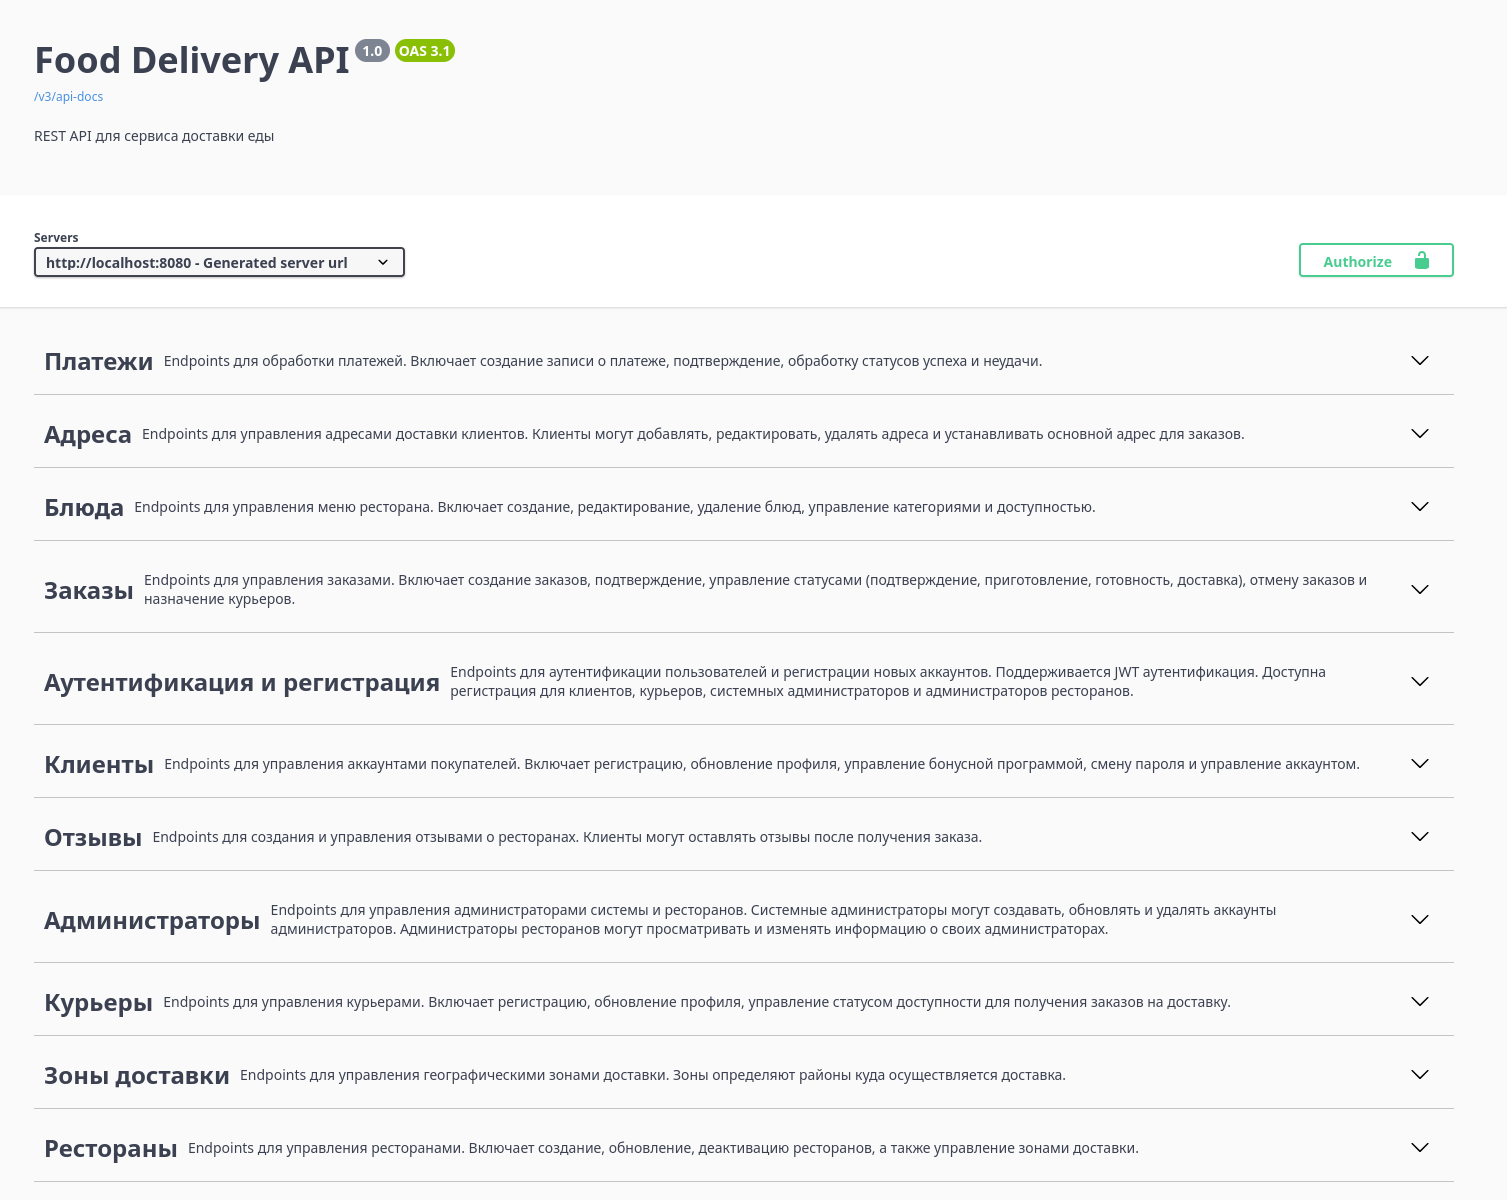
\includegraphics[width=\textwidth]{img/swagger_main.png}
    \caption{Главная страница Swagger UI}
    \label{img:swagger-main}
\end{figure}

На рисунке~\ref{img:swagger-request} представлен пример выполнения запроса на регистрацию клиента.

\begin{figure}[H]
    \centering
    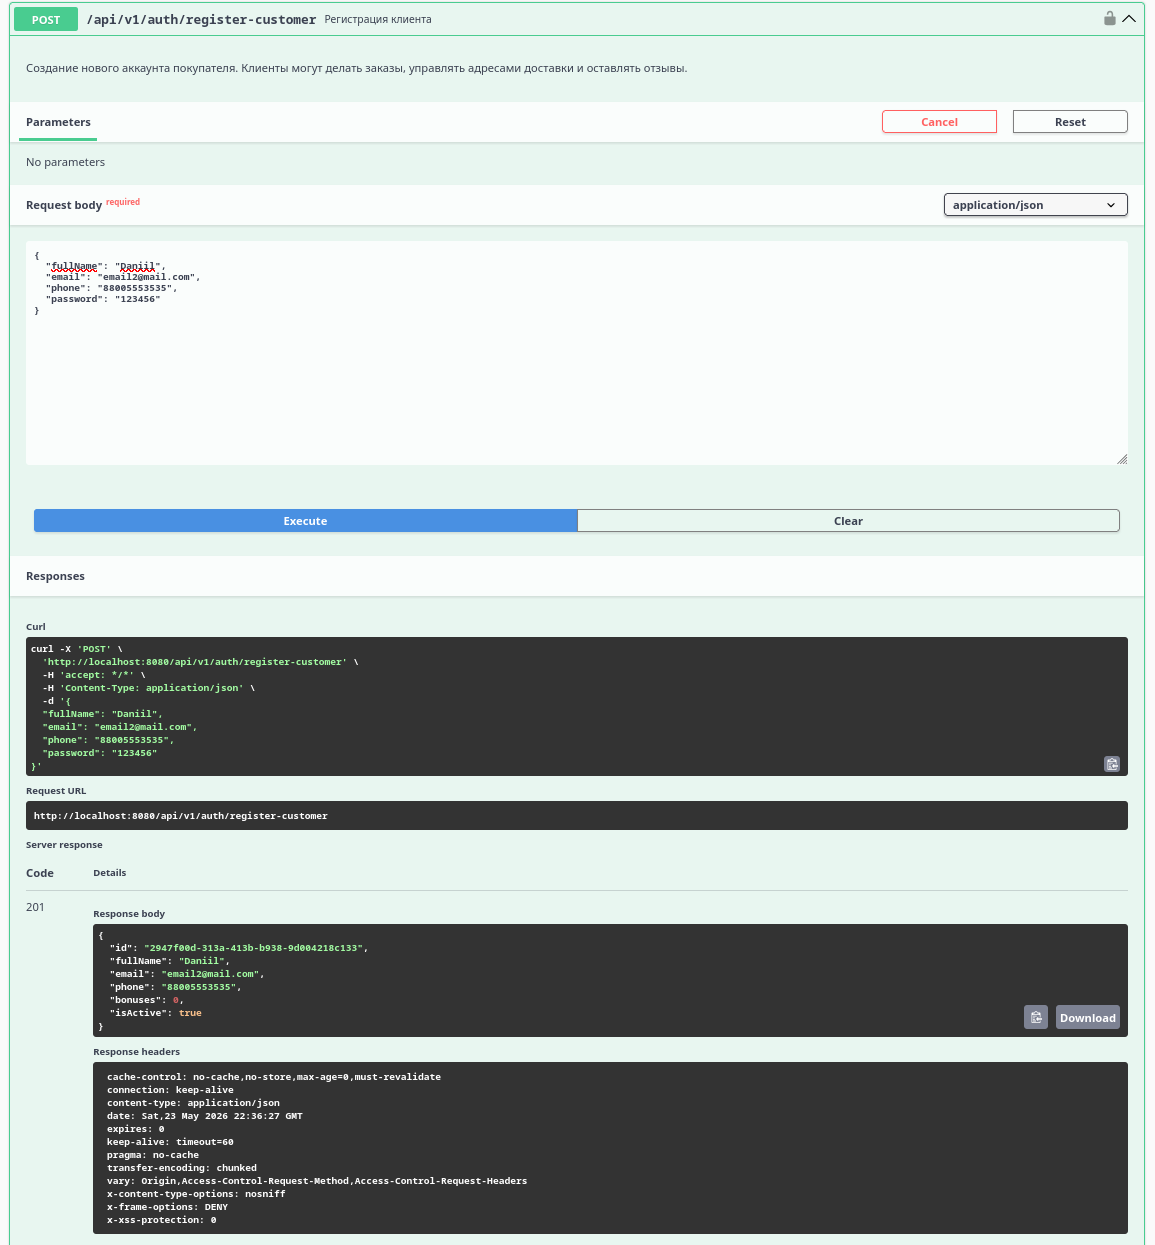
\includegraphics[width=\textwidth]{img/swagger_request.png}
    \caption{Пример выполнения запроса в Swagger UI}
    \label{img:swagger-request}
\end{figure}

\subsection{Вывод}
В технологическом разделе был обоснован выбор PostgreSQL в качестве основной СУБД, были созданы типы и таблицы базы данных и настроены ограничения их целостности. Разработаны функции и триггеры, а также приведены результаты их тестирования. Реализована ролевая модель разграничения прав доступа на уровне СУБД. На стороне приложения реализовано кэширование на базе СУБД Redis, дано описание взаимодействия Redis с PostgreSQL, и разработан интерфейс REST API с документацией в Swagger UI.